\documentclass[12pt,letterpaper]{report}
\usepackage{pgf, tikz}
\usetikzlibrary{arrows, automata,shapes.geometric,shapes.multipart}

\begin{document}
\tikzset{elliptic state/.style={draw,ellipse}}
    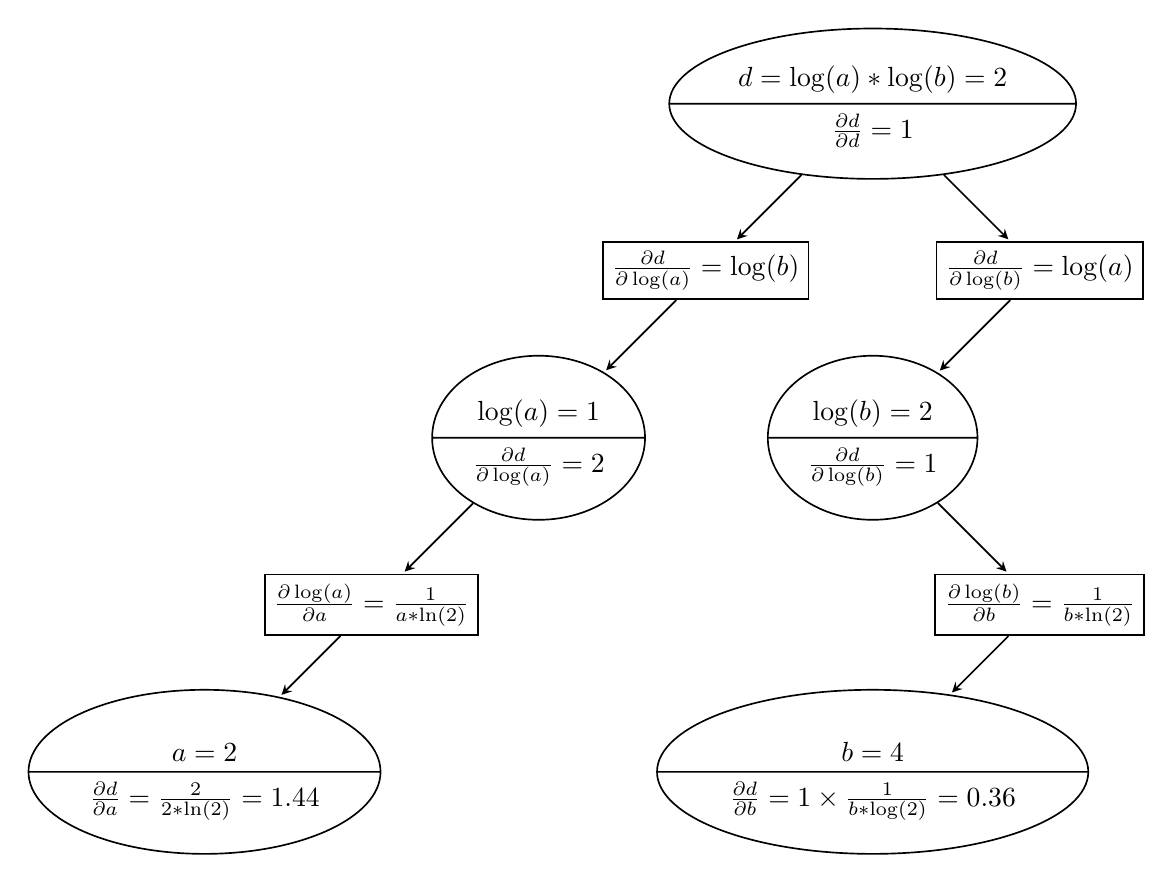
\begin{tikzpicture}[
            > = stealth, % arrow head style
            shorten > = 1pt, % don't touch arrow head to node
            auto,
            node distance = 3cm, % distance between nodes
            semithick % line style
        ]

        \tikzstyle{every state}=[
            draw = black,
            thick,
            fill = white,
            minimum size = 15mm
        ]

        \node[ellipse split, draw] (d) {
            $d=\log(a)*\log(b)=2$
            \nodepart{lower}
            $\frac{\partial d}{\partial d}=1$
            };
        %\node[align=center,anchor=south] (dlabel) at (d.south) {$\frac{\partial d}{\partial d}=1$};

         \node[rectangle,draw] (dloga) [below left of=d]{$\frac{\partial d}{\partial \log(a)}=\log(b)$};
         \node[rectangle,draw] (dlogb) [below right of=d]{$\frac{\partial d}{\partial \log(b)}=\log(a)$};
        
        \node[draw,ellipse split] (loga) [below left of=dloga]{
            
        $\log(a)=1$
        \nodepart{lower}
        $\frac{\partial d}{\partial \log(a)}=2$
        
        };
         %\node[align=center,anchor=south] (logalabel) at (loga.south) {$\frac{\partial d}{\partial \log(a)}=2$};

        \node[ellipse split, draw] (logb) [below left of=dlogb]{
            $\log(b)=2$
            \nodepart{lower}
            $\frac{\partial d}{\partial \log(b)}=1$
            
            };

        \node[rectangle,draw] (da) [below left of=loga]{$\frac{\partial \log(a)}{\partial a}=\frac{1}{a*\ln(2)}$};
        \node[rectangle,draw] (db) [below right of=logb]{$\frac{\partial \log(b)}{\partial b}=\frac{1}{b*\ln(2)}$};
       
        \node[ellipse split,draw] (a) [below left of=da] (a){
            $a=2$ 
            \nodepart{lower} 
            $\frac{\partial d}{\partial a}=\frac{2}{2*\ln(2)}=1.44$
            };
        %   \node [circle split,draw,double,fill=red!20] (a) [below left of=da]
        %   {
        %     % No \nodepart has been used, yet. So, the following is put in the
        %     % ``text'' node part by default.
        %     $q_1$
        %     \nodepart{lower} % Ok, end ``text'' part, start ``output'' part
        %     $00$
        %   }; % output part ended.
        %\node[align=center,anchor=south] (alabel) at (a.south) {$\frac{\partial d}{\partial a}=2*\frac{1}{2*\ln(2)}$};

        \node[ellipse split, draw] (b) [below left of=db]{
        $b=4$
        \nodepart{lower}
        $\frac{\partial d}{\partial b}=1\times\frac{1}{b*\log(2)}=0.36$
        };

       
         \path[->] (d) edge (dloga) ;
        \path[->] (d)  edge (dlogb);
         \path[->]  (dloga) edge (loga);
         \path[->]  (loga) edge (da);
         \path[->]  (da) edge (a);


         \path[->]  (dlogb) edge (logb);
         \path[->]  (logb) edge (db);
         \path[->]  (db) edge (b);
        % \path[->] (a) edge (ca);
        % \path[->] (db) edge (d);
        % \path[->] (b) edge (db);
        % \path[->] (d) edge (ed);
        % \path[->] (b) edge (cb);
        % \path[->] (a) edge (da);
        % \path[->] (da) edge (d);


        %\path[->] (s) edge node {18} (v1);
        %\path[->] (s) edge node {1} (v2);
        %\path[->] (s) edge node {1} (v3);
        %\path[->] (v2) edge node {2} (v1);
        %\path[->] (v3) edge node {1} (v2);
        %\path[->] (v1) edge node {20} (t);

        %\draw[red, dashed] (1, 2) -- (1, -2);
    \end{tikzpicture}

\end{document}